\documentclass[draft,linenumbers]{agujournal}
\draftfalse
\usepackage{hyperref}
\usepackage[export]{adjustbox}
\addtolength{\oddsidemargin}{-.875in}
\addtolength{\evensidemargin}{-.875in}
	
\hypersetup{
    colorlinks=true,
    linkcolor=blue,
    filecolor=magenta,      
    urlcolor=cyan,
}

\journalname{Journal of Advances in Modeling Earth Systems (JAMES)}

\begin{document}

\title{Supplementary Information for \emph{Parametric controls on vegetation responses to biogeochemical forcing in the CLM5} by Fisher et al. (submitted to JAMES)}

    \begin{figure}[h]
     \centering
     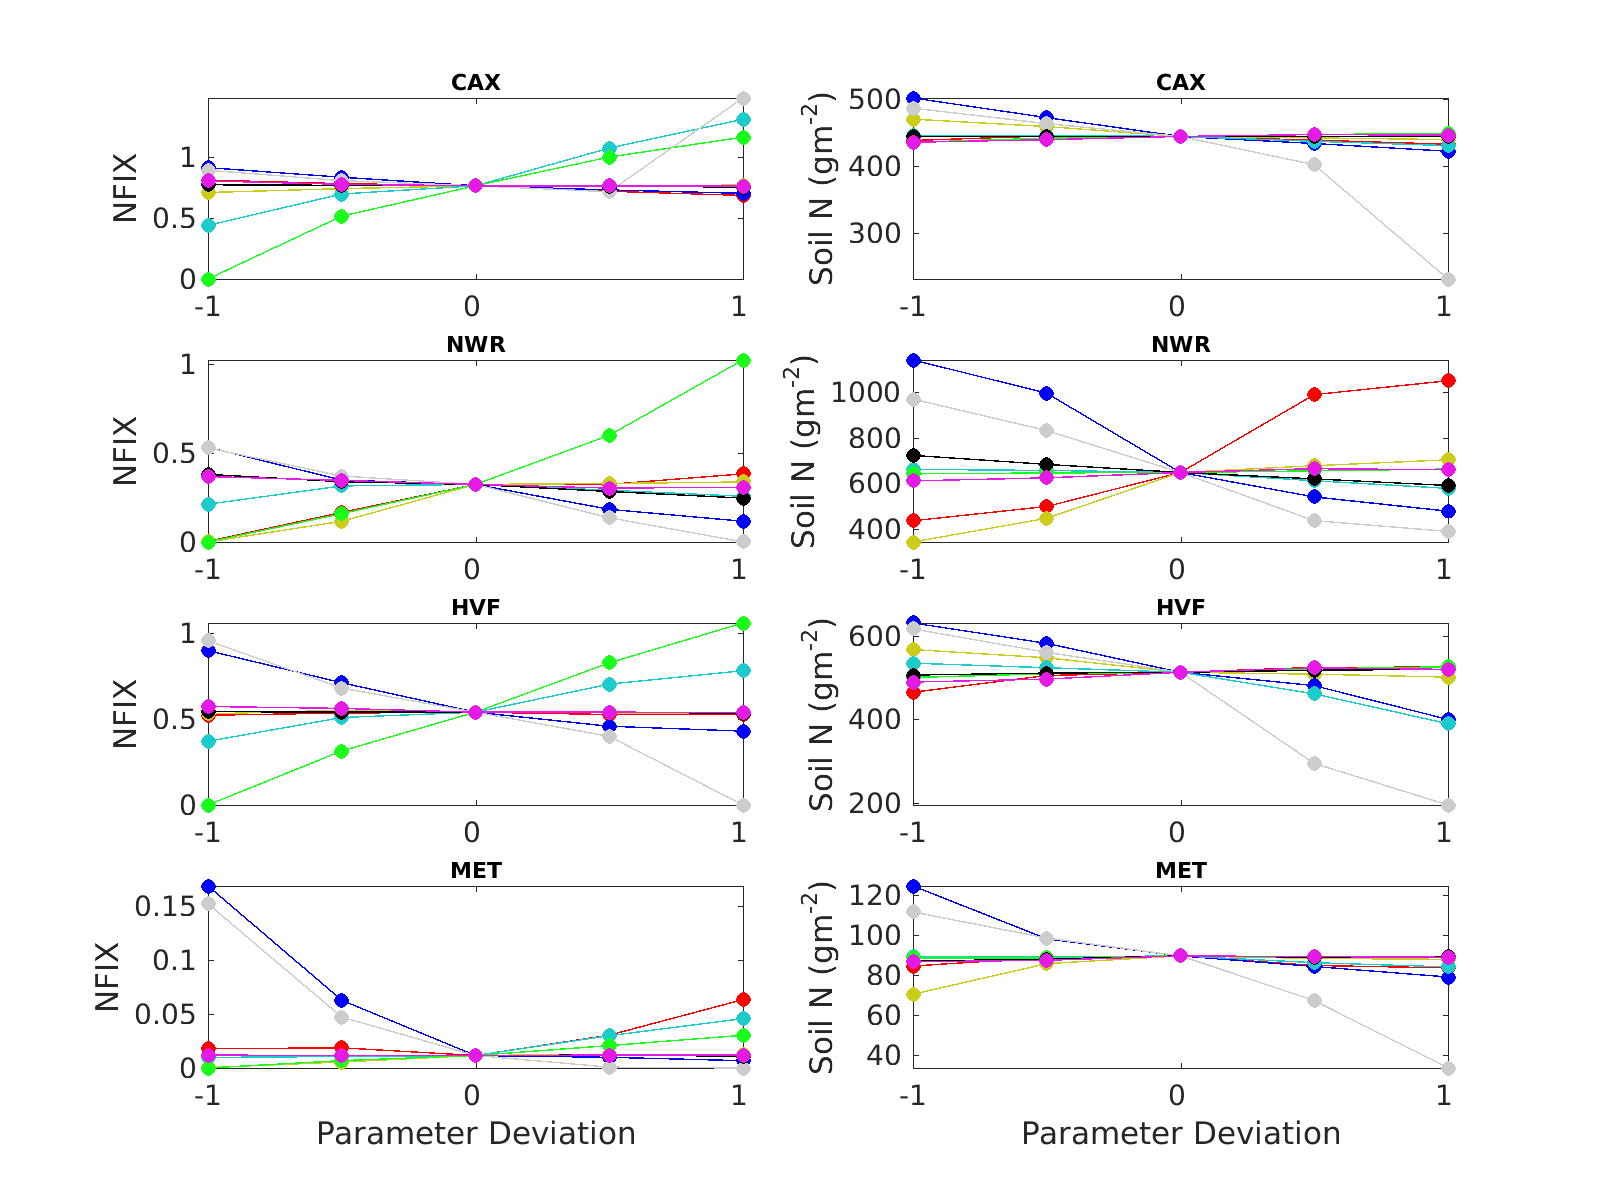
\includegraphics[width=1.0\textwidth, left]{matlab/figures/MAY19jp_MEANCOND_-r200_2013TOTSOMN.png}
     \caption{Influence of parametric variation   (over the range tested: -1 to +1, Table \ref{table_ranges}) on the model pre-fertilization state for Nitrogen fixation and total soil N content across the Caxiuan\~a (CAX), Niwot Ridge (NWR), Harvard Forest (HVF) and Metolious MET) sites.}
     \label{MEANSOM}
\end{figure}
  
\begin{figure}[h]
     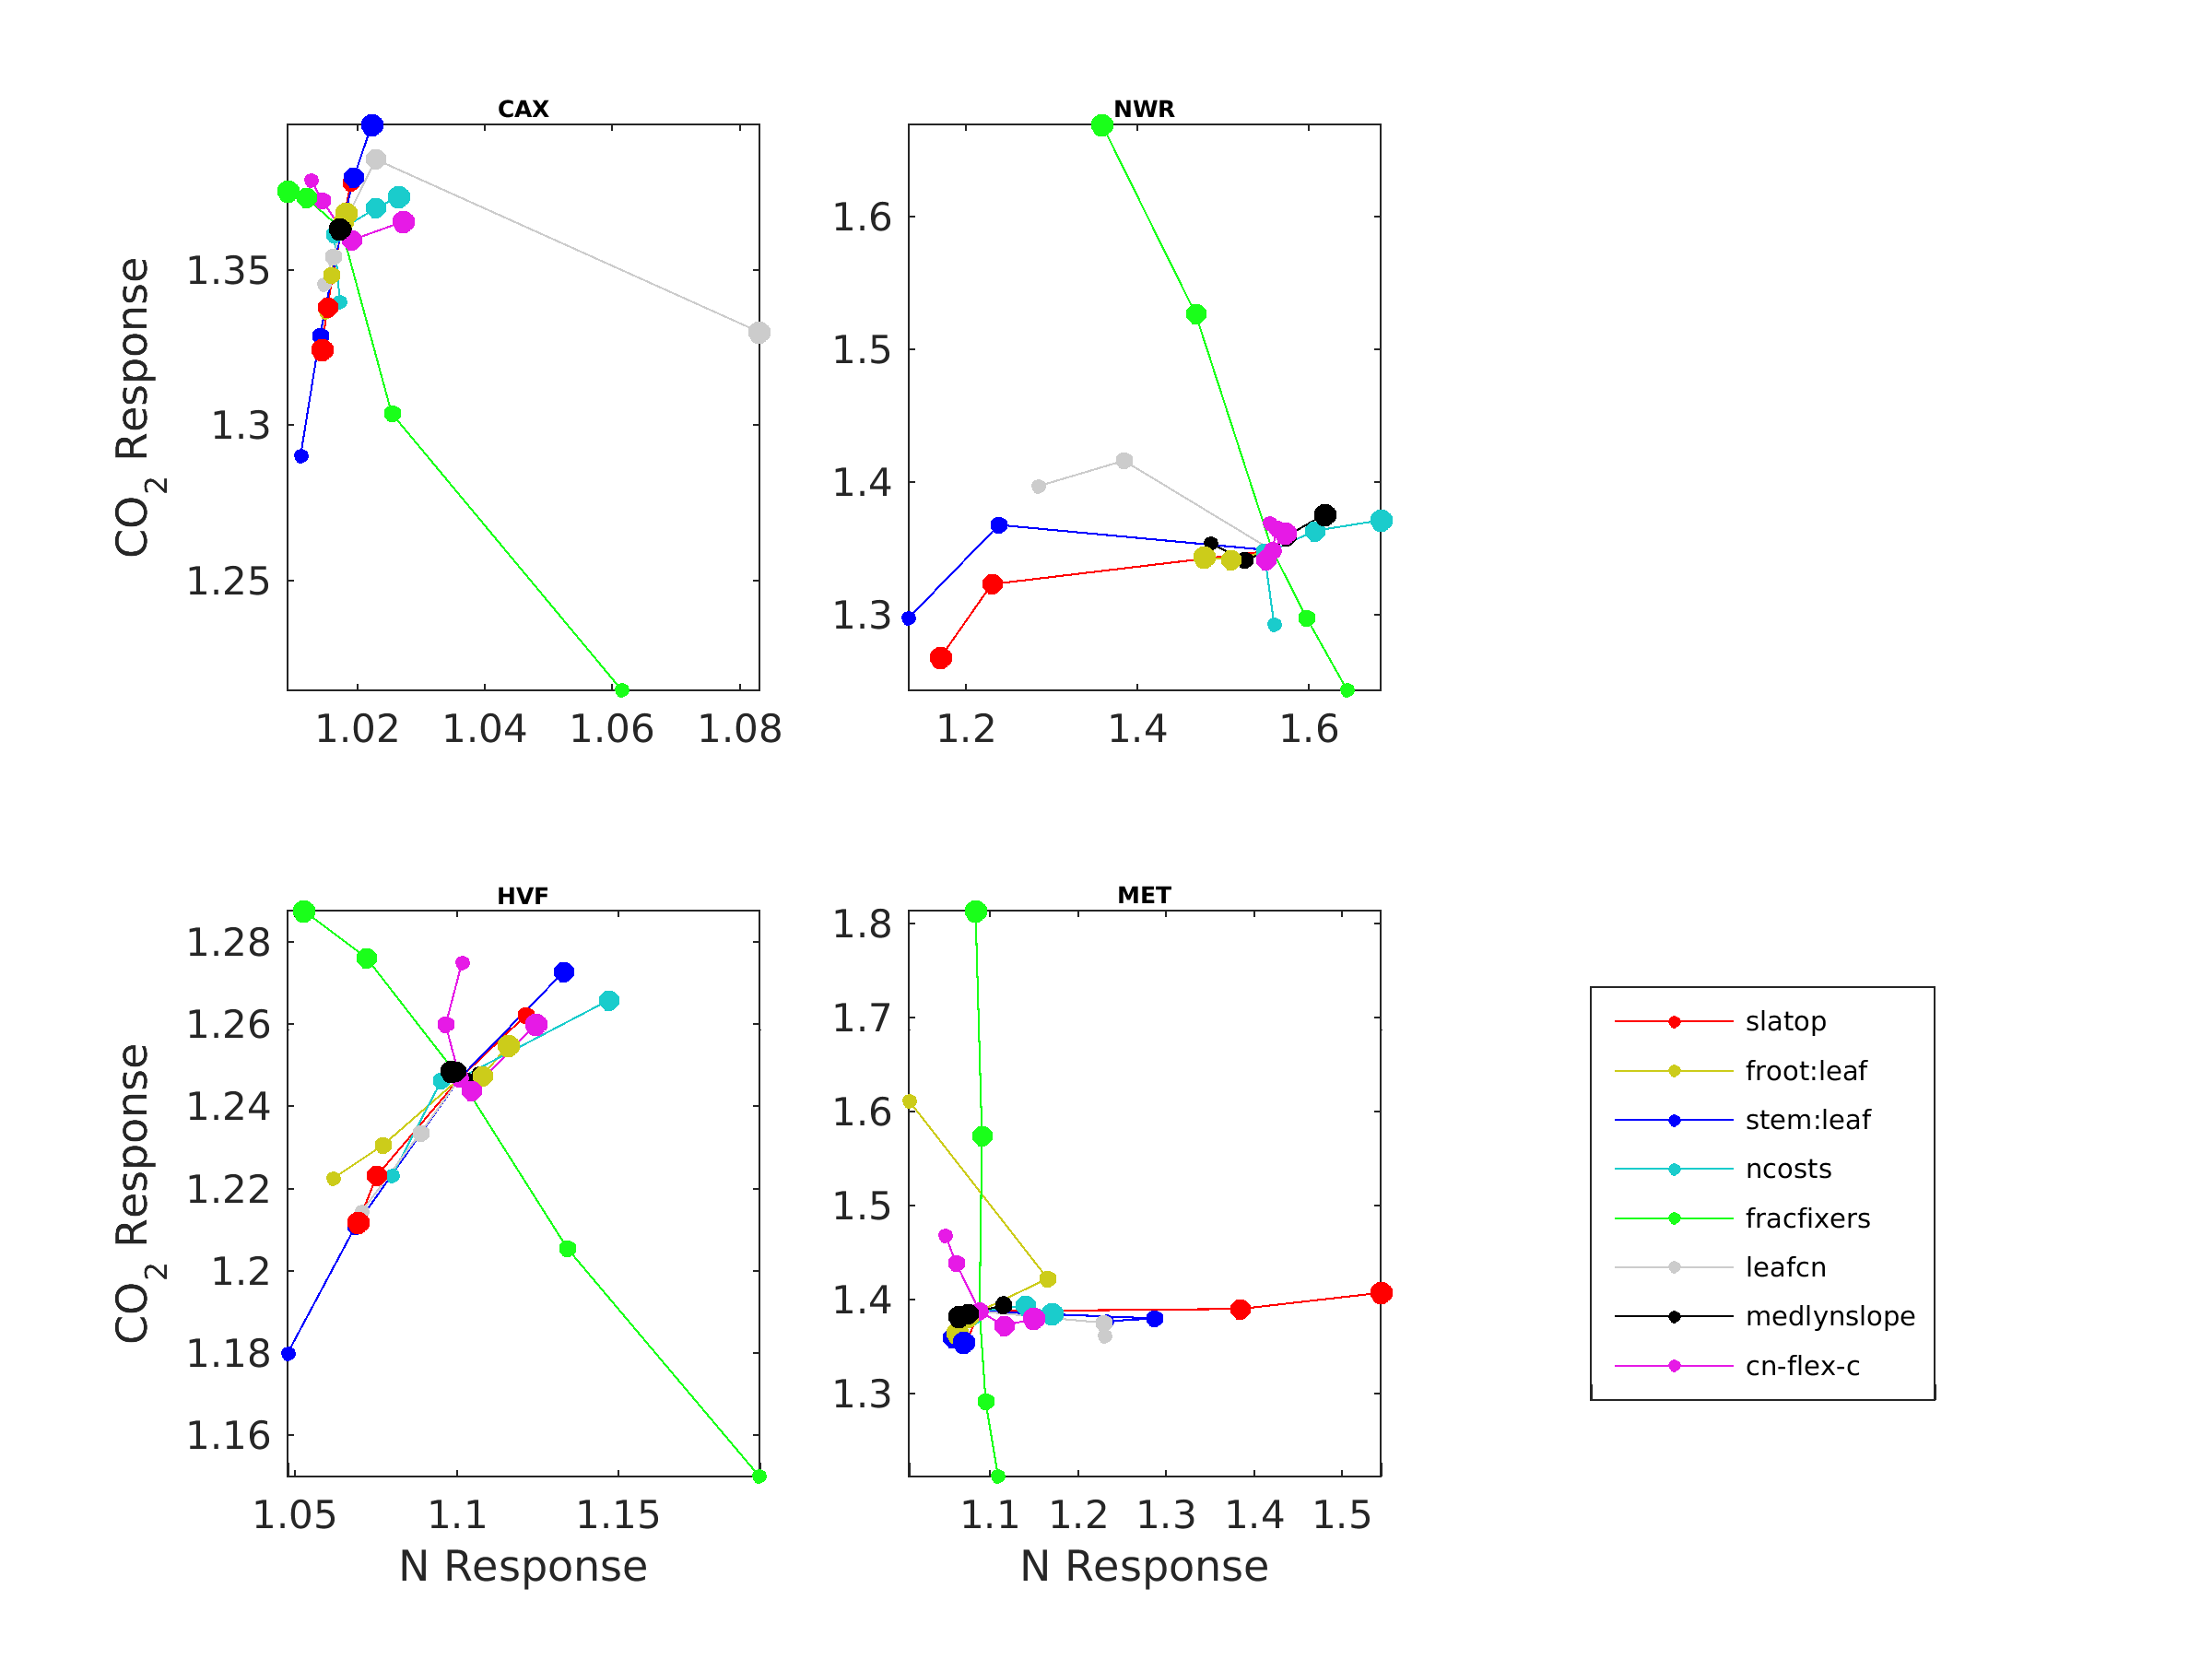
\includegraphics[width=1.2\textwidth]{matlab/figures/MAY19jp_at_relCNdep_defpft_TOTVEGC_y2013.png}
     \caption{Influence of parametric variation (over the range tested: -1 to +1, Table 1) on the model response (fertilized/control) to 15 years of 500ppm CO$_{2}$ and +5 Kg m$^{-2}$ y$^{-1}$ N fertilization, for net primary production (NPP)}
     \label{CN_NPP}
  \end{figure}
  
  
    \begin{figure}[h]
     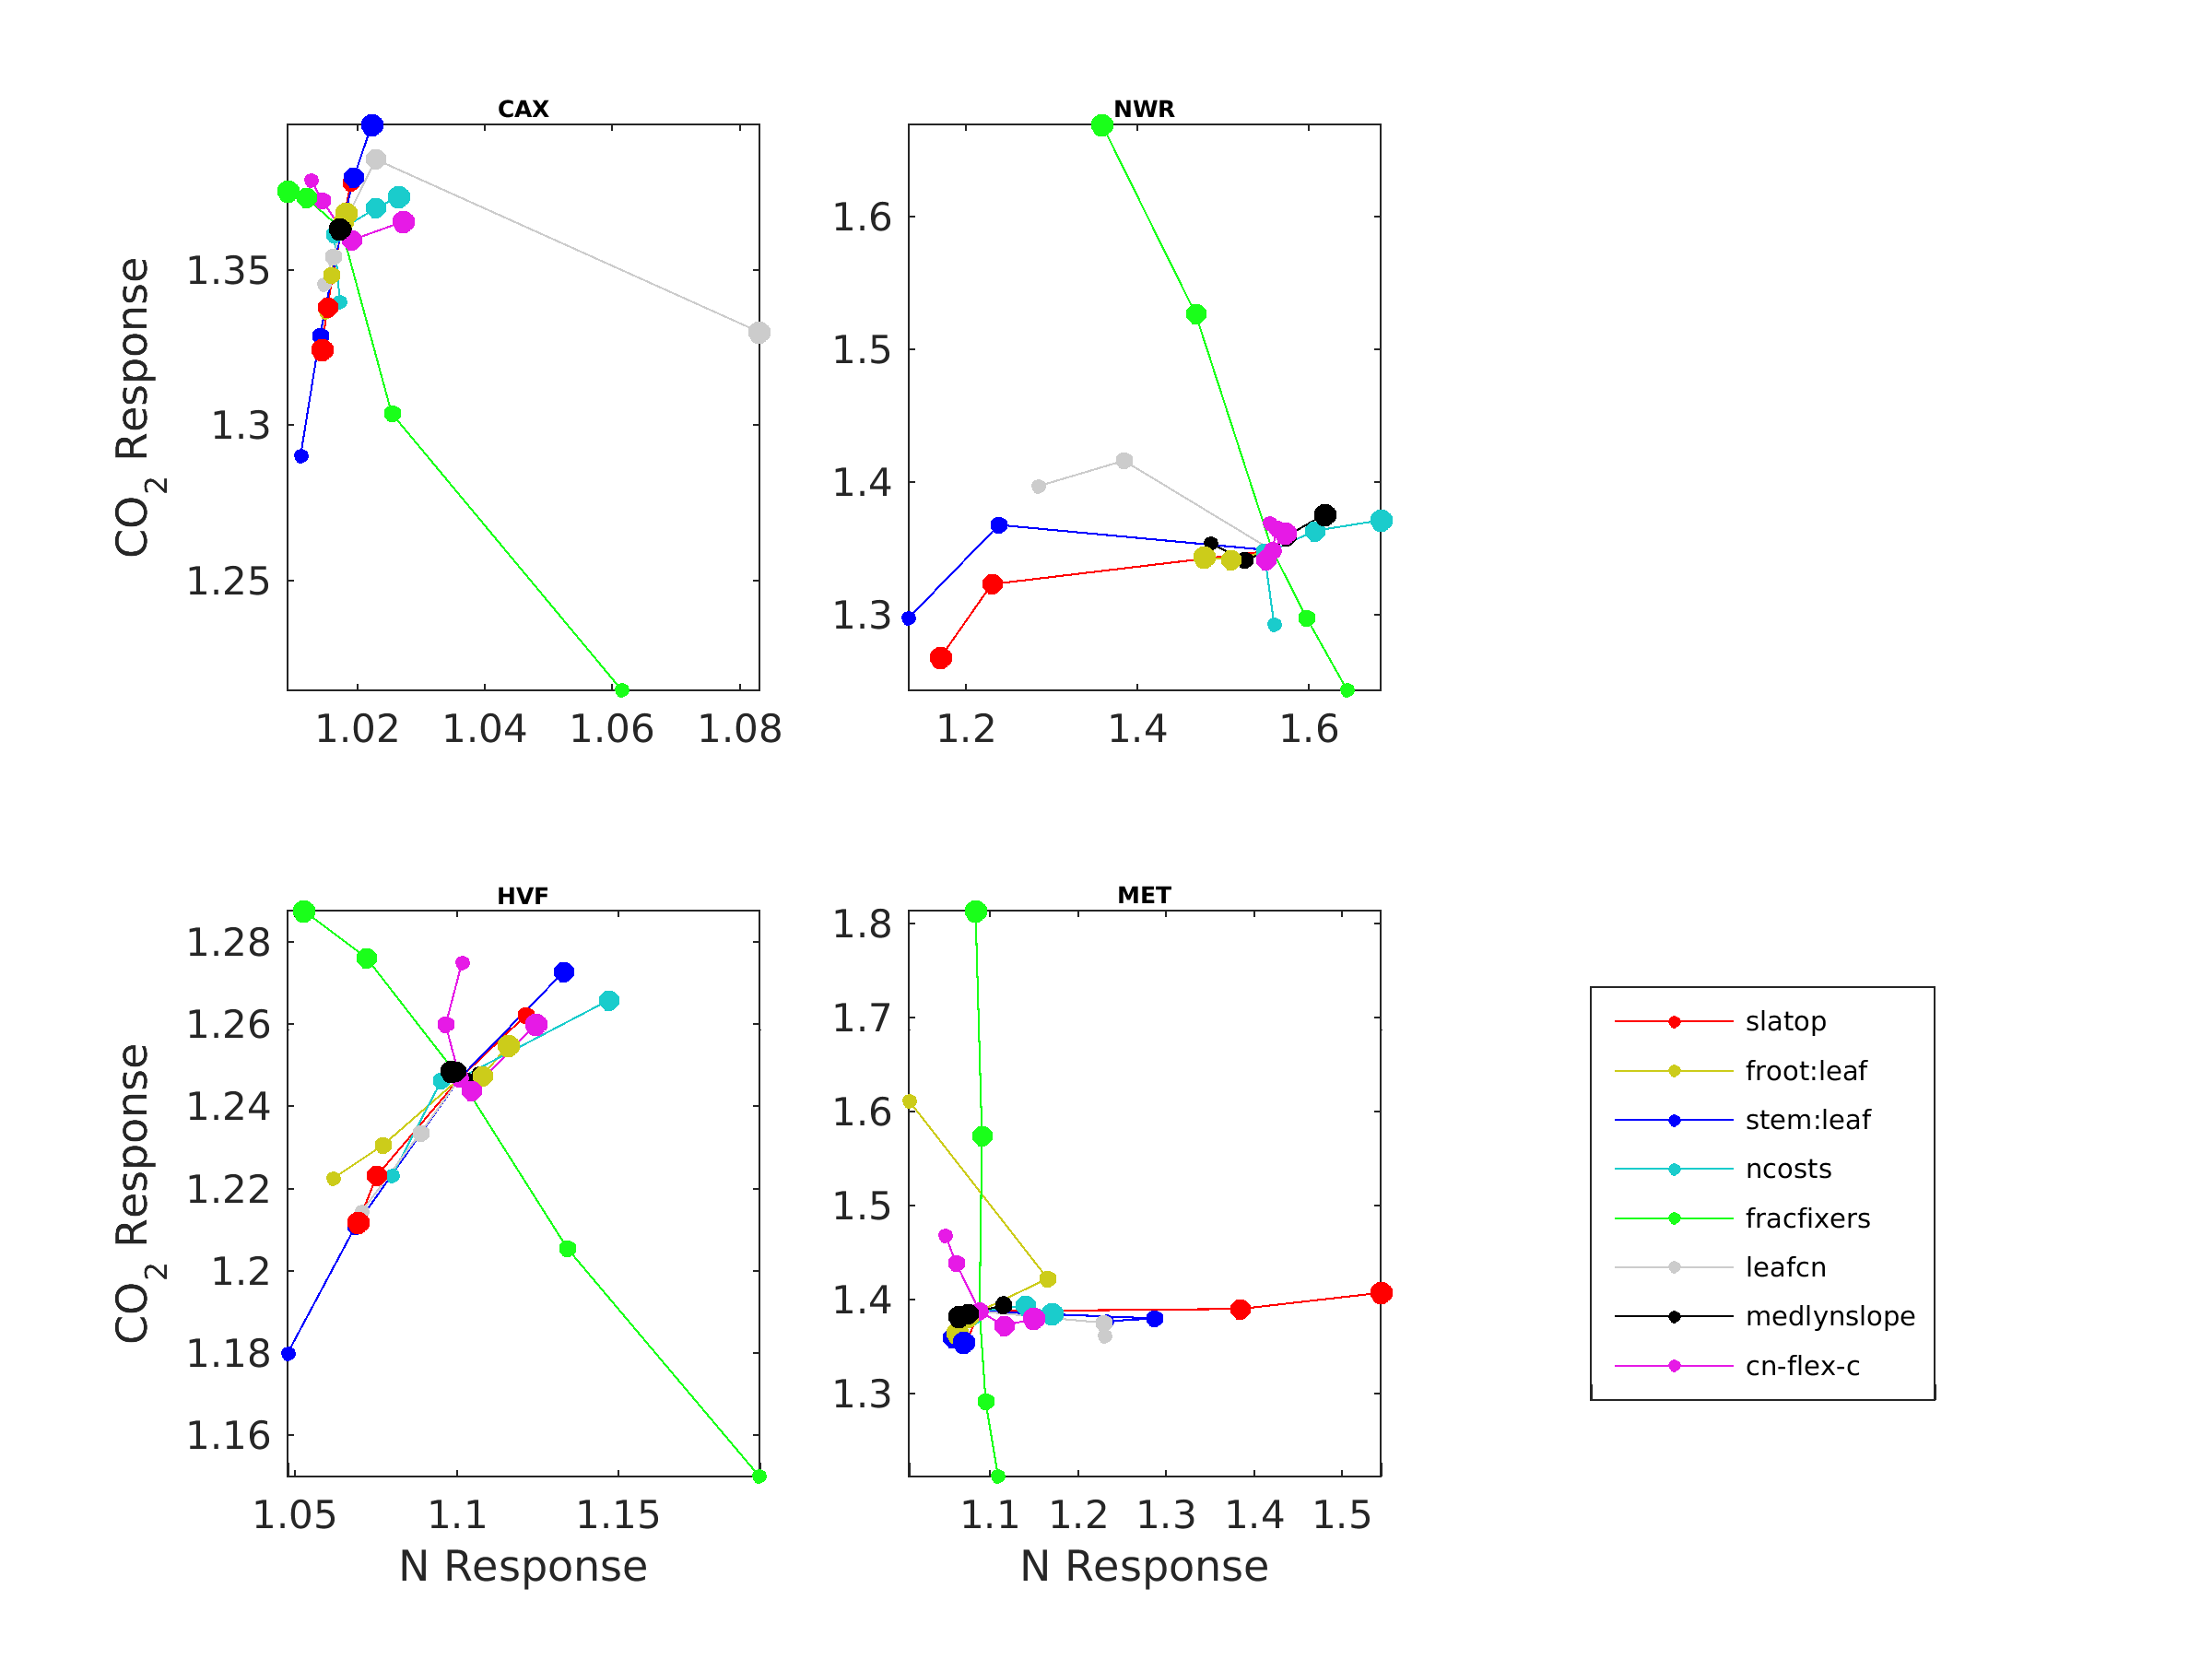
\includegraphics[width=1.2\textwidth]{matlab/figures/MAY19jp_at_relCNdep_defpft_TOTVEGC_y2013.png}
     \caption{Influence of parametric variation (over the range tested: -1 to +1, Table 1) on the model response (fertilized/control) to 15 years of 500ppm CO$_{2}$ and +5 Kg m$^{-2}$ y$^{-1}$ N fertilization, for total vegetation carbon)}
     \label{CN_TOTVEGC}
  \end{figure}
  
\begin{figure}[h]
     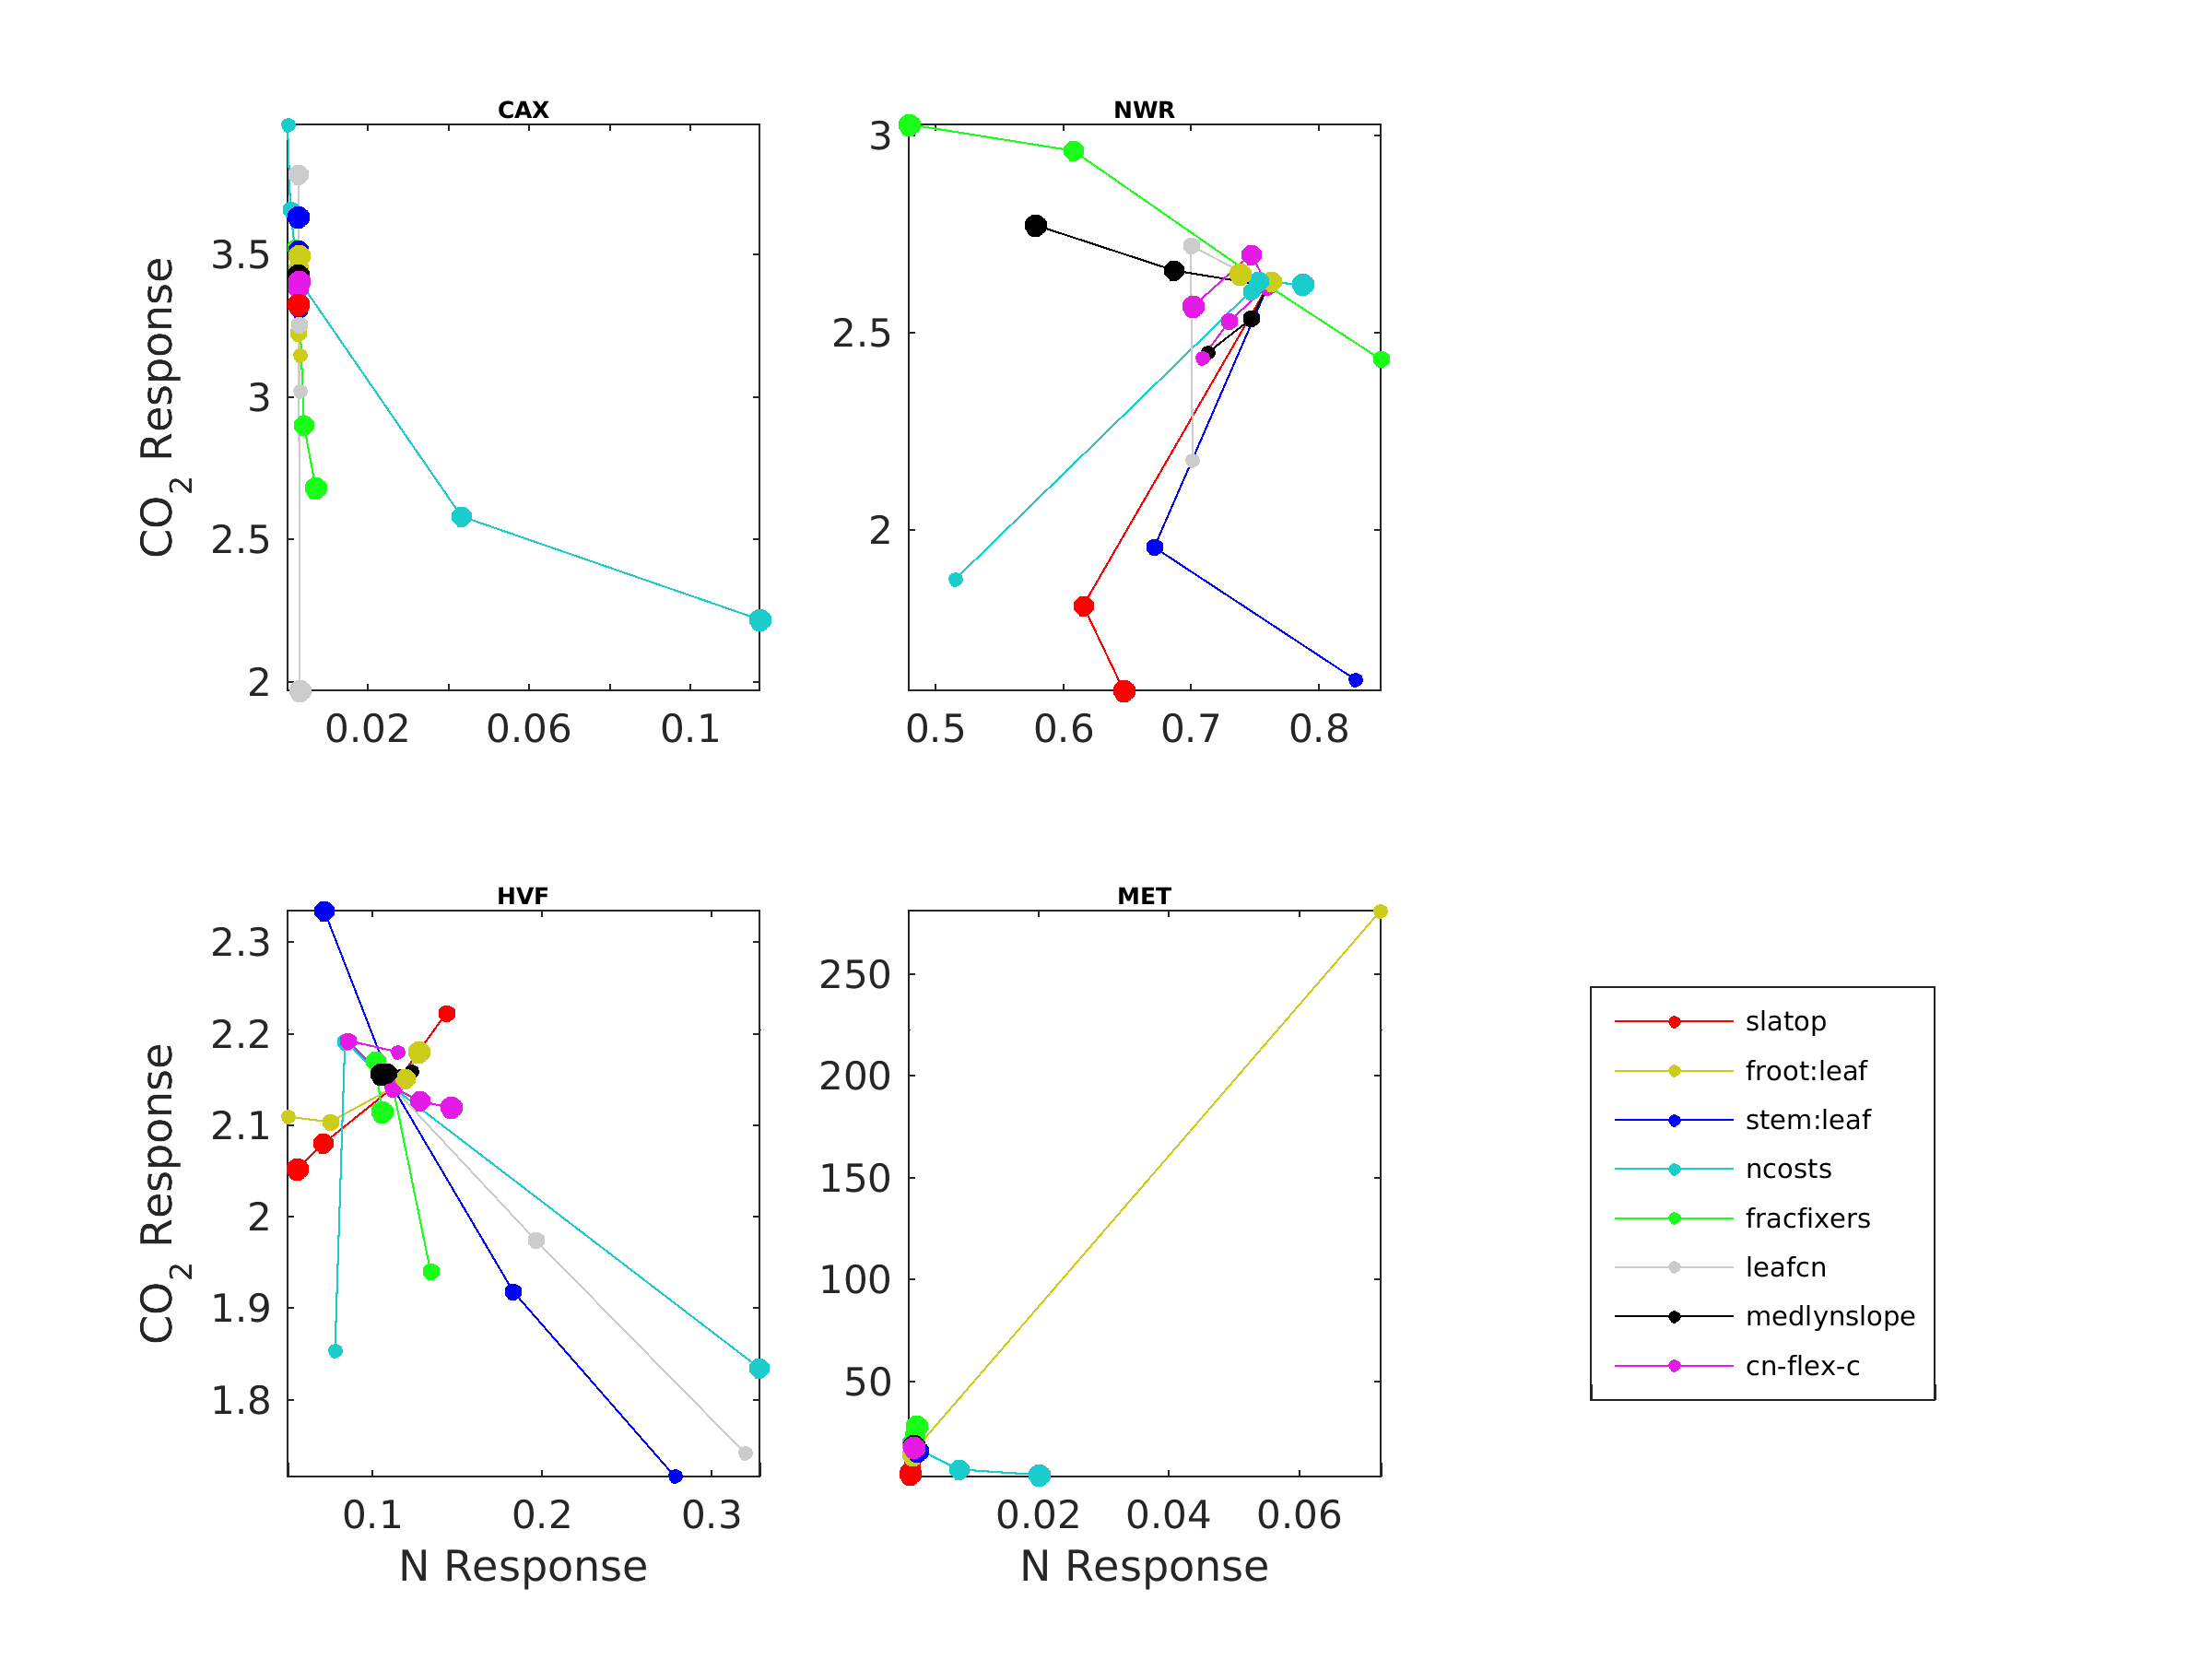
\includegraphics[width=1.2\textwidth]{matlab/figures/MAY19jp_at_relCNdep_defpft_NFIX_y2013.png}
     \caption{Influence of parametric variation (over the range tested: -1 to +1, Table 1) on the model response (fertilized/control) to 15 years of 500ppm CO$_{2}$ and +5 Kg m$^{-2}$ y$^{-1}$ N fertilization, for nitrogen fixation rates (NFIX, gN m^{-2})}
     \label{CN_NFIX}
  \end{figure}
  
  \begin{figure}[h]
     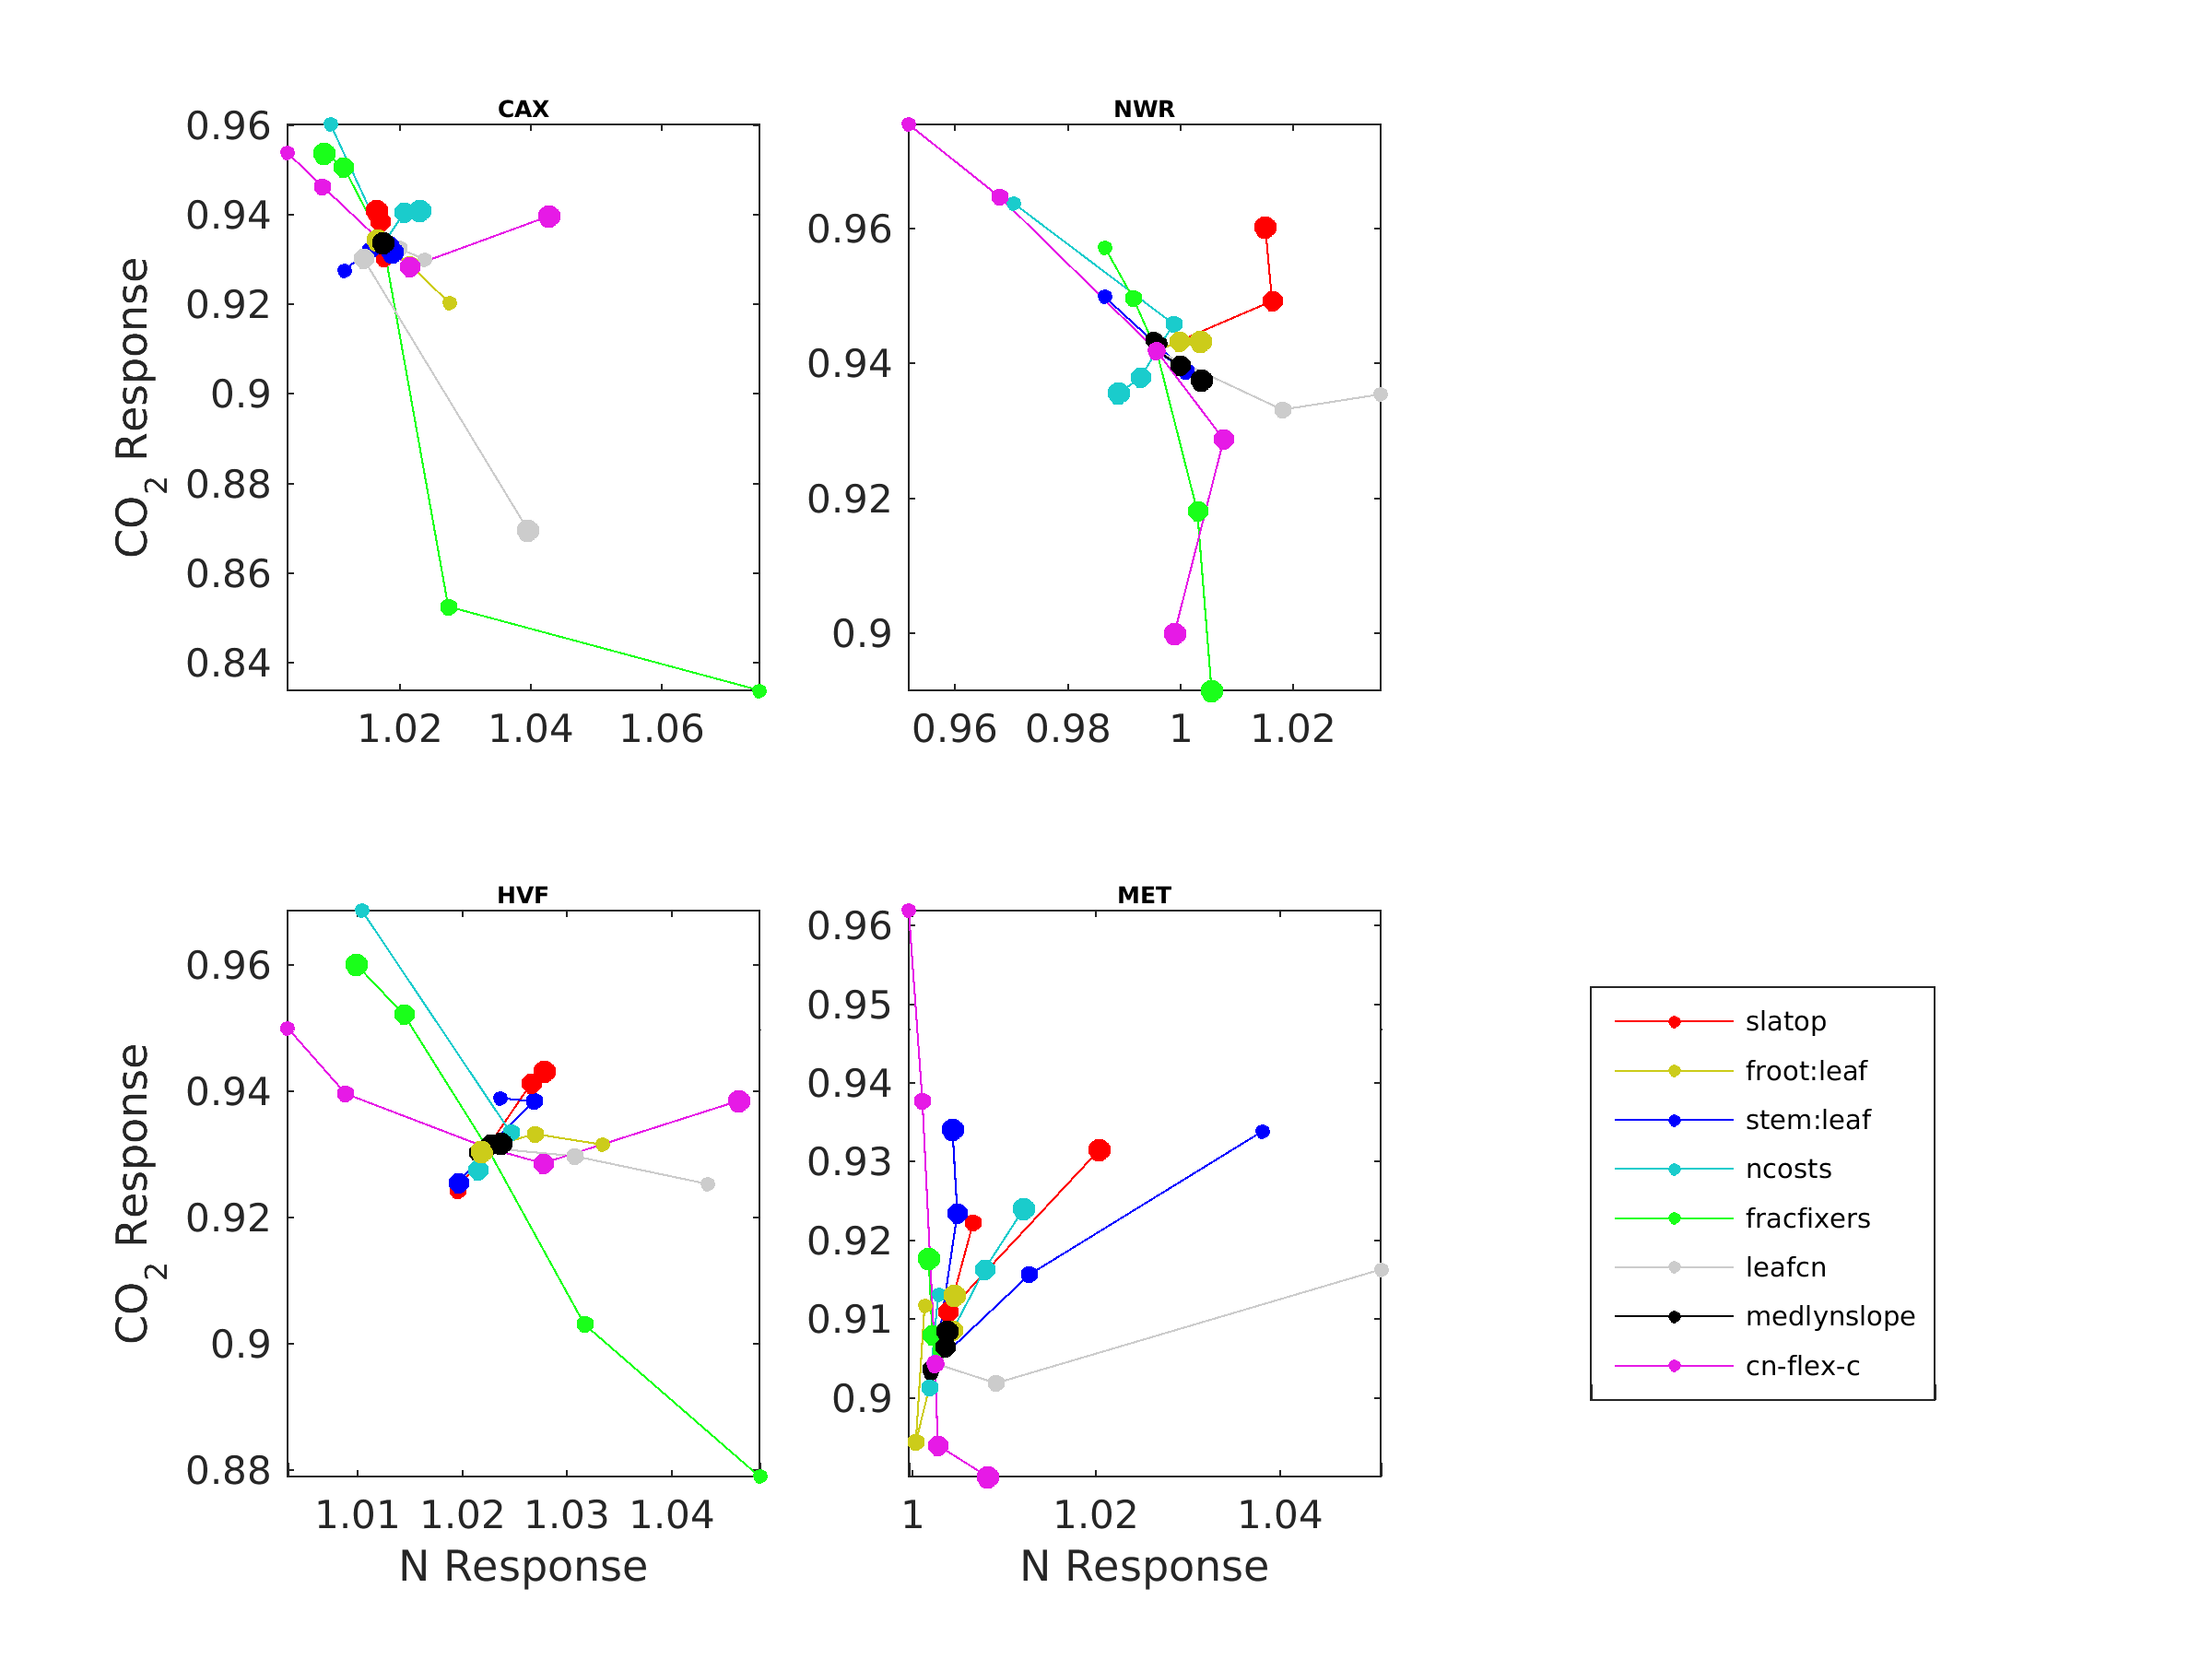
\includegraphics[width=1.2\textwidth]{matlab/figures/MAY19jp_at_relCNdep_defpft_LEAFN_y2013.png}
     \caption{Influence of parametric variation (over the range tested: -1 to +1, Table 1) on the model response (fertilized/control) to to 15 years of 500ppm CO$_{2}$ and +5 Kg m$^{-2}$ y$^{-1}$ N fertilization, for leaf nitrogen ($N_{leaf}$)}
     \label{CN_LEAFN}
  \end{figure}
 
 



\end{document}